\documentclass[mathserif,handout]{beamer}
%\documentclass{beamer}
\usetheme{metropolis}
\usepackage{amsmath,verbatim}
\usepackage{listings}
\usepackage{algorithmicx}
\usepackage{algpseudocode}
\usepackage[english]{babel}
%\usepackage{media9} % package for genuine embedding of movies
%\usepackage{multimedia} % beamer package for calling external files and players
\setbeamercovered{transparent}

% media9 stuff for playing movies
%\newcommand{\includemovie}[3]{\includemedia[width=#1,height=#2,activate=pagevisible,deactivate=pageclose,addresource=#3,flashvars={src=#3 &autoPlay=true &loop=true &controlBarAutoHideTimeout=0 }]{}{VPlayer.swf}}

\newcommand{\trans}{\ensuremath{{}^\mathrm{T}}}

\newcommand{\eps}{\varepsilon}
\newcommand{\reals}{\mathbb{R}}
\newcommand*{\approxdist}{\mathrel{\vcenter{\offinterlineskip
\vskip-.25ex\hbox{\hskip.55ex$\cdot$}\vskip-.25ex\hbox{$\sim$}
\vskip-.5ex\hbox{\hskip.55ex$\cdot$}}}}

\lstdefinelanguage{myR}
{
   language=R,
   otherkeywords={read.table, set.seed, head},
   deletekeywords={url,codes, t, dt, Call, formula,Q, R, on,by,hat,is,
col, set,start,end,deltat,zip},
   sensitive=true,
   breaklines=true,
   morecomment=[l]{\#},
   morestring=[b]",
   morestring=[b]',
   basicstyle =\ttfamily\small,
   keywordstyle=\bfseries,
   showtabs=false,
   showstringspaces=false,
   literate= {~}{$\sim$}{2},
   numberstyle=\sffamily\scriptsize,
   stepnumber=2
 }

% \lstset{basicstyle=\ttfamily\color{blue}}
% \lstset{language=scala, basicstyle=\ttfamily\small, breaklines=true}

\definecolor{dkgreen}{rgb}{0,0.2,0}
\definecolor{dkblue}{rgb}{0,0,0.6}

\lstdefinelanguage{scala}{
  morekeywords={abstract,case,catch,class,def,%
    do,else,extends,false,final,finally,%
    for,if,implicit,import,match,mixin,%
    new,null,object,override,package,%
    private,protected,requires,return,sealed,%
    super,this,throw,trait,true,try,%
    type,val,var,while,with,yield},
  otherkeywords={=>,<-,<\%,<:,>:,\#,@},
  sensitive=true,
  basicstyle =\ttfamily\small\color{dkblue},
  keywordstyle=\sffamily\bfseries\color{dkgreen},
  morecomment=[l]{//},
  morecomment=[n]{/*}{*/},
  morestring=[b]",
  morestring=[b]',
  morestring=[b]"""
}

\lstMakeShortInline[language=scala]|


\newcommand*\Let[2]{\State #1 $\gets$ #2}
\newcommand*\Draw[2]{\State \textbf{draw} #1 $\sim$ #2}

\begin{document}

\title{A compositional approach to scalable Bayesian computation and probabilistic programming}
\author[Darren Wilkinson --- Cambridge 14/12/18]{\textbf{\large Darren Wilkinson} \\
\url{@darrenjw}\hfill \alert{\url{darrenjw.github.io}}\\
\vspace{2ex}%
%School of Mathematics, Statistics and Physics\\
Newcastle University, UK / The Alan Turing Institute}
\date{\textbf{Advances and challenges in machine learning languages}\\\emph{Cambridge University}\\20-21 May 2019}

  
\frame{\titlepage}


\frame{
  \frametitle{Overview}
  \vfill
  \vfill
  \tableofcontents
}

\begin{comment}

  \frame{
  \frametitle{Aside: SMfSB3e just published!}
  \begin{minipage}{0.45\textwidth}
    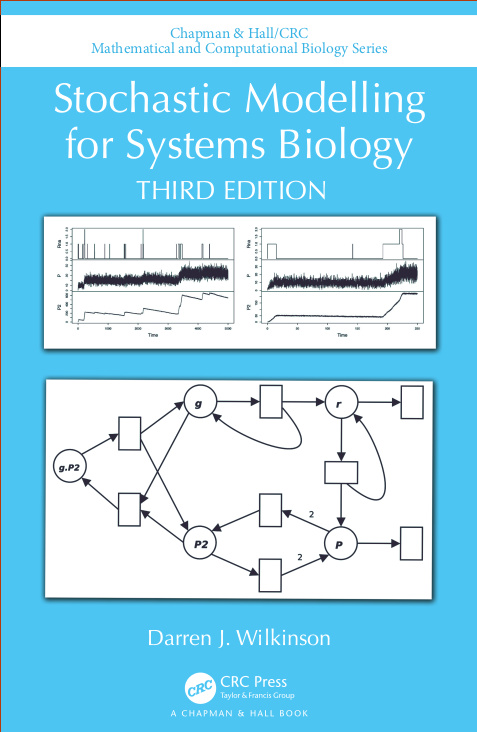
\includegraphics[height=0.8\textheight]{cover-3e}
  \end{minipage}
  \begin{minipage}{0.48\textwidth}
    \begin{itemize}
    \item New chapter on stochastic reaction--diffusion models
      \item Extended chapter on inference: pMCMC, ABC, ABC--SMC, ...
      \item New website/GitHub repository
        \item Lots of new, improved and updated software --- all free, open source and well-documented
    \end{itemize}
  \end{minipage}\\
  \vspace{2ex}
    \centerline{\alert{\url{https://github.com/darrenjw/smfsb}}}
  }



\section{Background}

\frame{
  \frametitle{Changing face of statistics}
  \begin{itemize}
  \item The practice of academic statistics, and especially computational statistics, has changed beyond recognition in the last 40 years
  \item It is likely to change even more in the next 40 years
  \item This is the age of data...
  \item Boundaries are blurring between \alert{statistics} and related disciplines, such as \alert{machine learning}, \alert{AI}, and \alert{data science}
  \item Computing and computational approaches are progressing very rapidly in all of these disciplines, and this is impacting how we do and think about computing in statistics
  \item Most people in these other fields don't use R
    \item Will we still be using R in 20 years time? I doubt it, and I really hope not!
    \end{itemize}
  }

\frame{
  \frametitle{What's up with statistical computing?}
  \begin{itemize}
    \pause
  \item Everything!
    \pause
  \item \alert{R} has become the de facto standard programming language for statistical computing --- the S language was designed by statisticians for statisticians in the mid 1970's, and it shows!
    \pause
    \begin{itemize}
    \item Many dubious language design choices, meaning it will always be ugly, slow and inefficient (without many significant breaking changes to the language)
    \item R's inherent inefficiencies mean that much of the R code-base isn't in R at all, but instead in other languages, such as \alert{Fortran}, \alert{C} and \alert{C++}
      \item Although faster and more efficient than R, these languages are actually all even \alert{worse} languages for statistical computing than~R!
      \end{itemize}
  \end{itemize}
  }

\frame{
  \frametitle{Pre-historic programming languages}
  \begin{itemize}
  \item All of the programming languages commonly used for scientific and statistical computing were designed 30-50 years ago, in the dawn of the computing age, and haven't significantly changed
    \begin{itemize}
  \item Compare with how much computing \alert{hardware} has changed in the last 40 years!
  \item But the language you are using was designed for that hardware using the knowledge of programming languages that existed at that time
  \item Think about how much \alert{statistical methodology} has changed in the last 40 years --- you wouldn't use 40 year old methodology --- why use 40 year old languages to implement it?!
    \end{itemize}
    \end{itemize}
}


\end{comment}

\section{Compositionality, category theory, and functional programming}

\subsection{Compositionality}



\frame{
\frametitle{Compositionality and modelling}
\begin{itemize}
\item We typically solve big problems by (recursively) breaking them down into smaller problems that we can solve more easily, and then \alert{compose} the solutions of the smaller problems to provide a solution to the big problem that we are really interested in
\item This \alert{``divide and conquer''} approach is necessary for the development of genuinely \alert{scalable} models and algorithms
\item Statistical models and algorithms are not usually formulated in a composable way
\item \alert{Category theory} is in many ways the \alert{mathematical study of composition}, and provides significant insight into the development of more compositional models of computation
\end{itemize}
}

\begin{comment}

\frame{
\frametitle{Compositionality and programming}
\begin{itemize}
\item The programming languages typically used for scientific and statistical computing also fail to naturally support composition of models, data and computation
\item Functional programming languages which are strongly influenced by category theory turn out to be much better suited to the development of scalable statistical algorithms than the imperative programming languages more commonly used
\item Expressing algorithms in a functional/categorical way is not only more elegant, concise and less error-prone, but provides numerous more tangible benefits, such as automatic parallelisation and distribution of algorithms
\end{itemize}
}

\begin{frame}[fragile]
  \frametitle{Imperative pseudo--code}
  \begin{minipage}{5.5cm}
  \begin{algorithmic}[1]
    \Function{MonteC}{$n$}
    \Let{$x$}{$0$}
    \For{$i \gets 1 \textrm{ to } n$}
    \Draw{$u$}{$U(0,1)$}
    \Draw{$v$}{$U(0,1)$}
    \If{$u^2+v^2<1$}
    \Let{$x$}{$x+1$}
    \EndIf
    \EndFor
    \State \Return{$4x/n$}
    \EndFunction
  \end{algorithmic}
  \end{minipage}
%\end{frame}
%\begin{frame}[fragile]
%  \frametitle{Imperative pseudo--code}
  \begin{minipage}{5cm}
  \begin{algorithmic}[1]
    \Function{Metrop}{$n,\eps$}
    \Let{$x$}{$0$}
    \For{$i \gets 1 \textrm{ to } n$}
    \Draw{$z$}{$U(-\eps,\eps)$}
    \Let{$x'$}{$x+z$}
    \Let{$A$}{$\phi(x')/\phi(x)$}
    \Draw{$u$}{$U(0,1)$}
    \If{$u<A$}
    \Let{$x$}{$x'$}
    \EndIf
    \EndFor
    \State \Return{$x$}
    \EndFunction
  \end{algorithmic}
  \end{minipage}

  \bigskip
  Not obvious that one of these is naturally parallel\ldots
\end{frame}


\frame{
  \frametitle{Modern programming language design}
  \begin{itemize}
  \item We have learned just as much about programming and programming languages in the last 40 years as we have about everything else
  \item Our understanding has developed in parallel with developments in hardware
  \item People have been thinking a lot about how languages can and should exploit modern computing hardware such as multi-core processors and parallel computing clusters
    \item Modern functional programming languages are emerging as better suited to modern hardware
    \end{itemize}
  }

\end{comment}

%\section{FP and CT}

\subsection{Functional Programming}

\frame{
  \frametitle{What is functional programming?}
  \begin{itemize}
  \item FP languages emphasise the use of \alert{immutable} data, \alert{pure}, \alert{referentially transparent functions}, and \alert{higher-order functions}
  \item Unlike commonly used \alert{imperative} programming languages, they are closer to the Church end of the \alert{Church-Turing thesis} --- eg. closer to \alert{Lambda--calculus} than a \alert{Turing--machine}
  \item The original Lambda--calculus was \alert{untyped}, corresponding to a \alert{dynamically--typed} programming language, such as \alert{Lisp}
    \item \alert{Statically--typed} FP languages (such as \alert{Haskell}) are arguably more scalable, corresponding to the \alert{simply--typed Lambda--calculus}, closely related to \alert{Cartesian closed categories}...
  \end{itemize}
  }

\begin{comment}

\frame{
  \frametitle{Functional programming}
  \begin{itemize}
  \item In pure FP, all state is \alert{immutable} --- you can assign names to things, but you can't change what the name points to --- no ``variables'' in the usual sense
  \item Functions are \alert{pure} and \alert{referentially transparent} --- they can't have side-effects --- they are just like functions in mathematics...
  \item Functions can be recursive, and \alert{recursion} can be used to iterate over recursive data structures --- useful since no conventional ``for'' or ``while'' loops in pure FP languages
  \item Functions are first class objects, and \alert{higher-order functions} (HOFs) are used extensively --- functions which return a function or accept a function as argument
  \end{itemize}
  }

\begin{frame}[fragile]
  \frametitle{Concurrency, parallel programming and shared mutable state}
  \begin{itemize}
  \item Modern computer architectures have processors with several cores, and possibly several processors
  \item Parallel programming is required to properly exploit this hardware
  \item The main difficulties with parallel and concurrent programming using imperative languages all relate to issues associated with \alert{shared mutable state}
  \item In pure FP, state is not mutable, so there is no mutable state, and hence no shared mutable state
    \item Most of the difficulties associated with parallel and concurrent programming just don't exist in FP --- this has been one of the main reasons for the recent resurgence of FP languages
  \end{itemize}
\end{frame}

  
\frame{
  \frametitle{Ideal languages for statistical computing}
  \begin{itemize}
  \item We should approach the problem of statistical modelling and efficient computation in a modular, composable, functional way
  \item To do this we need programming languages which are:
    \begin{itemize}
    \item \alert{Strongly statically typed} (but with type inference)
    \item \alert{Compiled} (but possibly to a VM)
    \item \alert{Functional} (with support for immutable values, immutable collections, ADTs and higher-order functions)
      \item and have support for \alert{typeclasses} and \alert{higher-kinded types}, allowing the adoption of design patterns from \alert{category theory}
    \end{itemize}
  \item For efficient statistical computing, it can be argued that evaluation should be \alert{strict} rather than \alert{lazy} by default
    \item \alert{Scala} is a popular language which meets the above constraints
  \end{itemize}
  }

\end{comment}

\begin{frame}[fragile]
  \frametitle{Monadic collections (in Scala)}
  \begin{itemize}
  \item A collection of type |M[T]| can contain (multiple) values of type~|T|
  \item If the collection supports a higher-order function\\
    |map(f: T => S): M[S]| then we call the collection a \alert{Functor}
    \begin{itemize}
    \item eg. |List(1,3,5,7) map (x => x*2) = List(2,6,10,14)|
    \end{itemize}
  \item If the collection additionally supports a higher-order function\\
    |flatMap(f: T => M[S]): M[S]| then we call the collection a \alert{Monad}
    \begin{itemize}
    \item eg. |List(1,3,5,7) flatMap (x => List(x,x+1))|\\
      \hspace{6ex} |= List(1, 2, 3, 4, 5, 6, 7, 8)|
    \item instead of |List(1,3,5,7) map (x => List(x,x+1))|\\
      |= List(List(1,2),List(3,4),List(5,6),List(7,8))|
    \end{itemize}
  \end{itemize}
\end{frame}

\begin{comment}
  
\begin{frame}[fragile]
  \frametitle{Other monadic types: Option}
  \begin{itemize}
  \item Some computations can fail, and we can capture that possibility with a type called |Option|
    \begin{itemize}
    \item in Scala --- it is |Optional| in Java 8 and |Maybe| in Haskell
      \end{itemize}
    \item An |Option[T]| can contain |Some[T]| or |None|
    \item So if we have |chol: Matrix => Option[TriMatrix]| we can check to see if we have a result
    \item But if we also have |triSolve: (TriMatrix,Vector) => Option[Vector]|, how do we ``compose'' these?
      \begin{itemize}
      \item |chol(mat) map (tm => triSolve(tm,vec))| has type |Option[Option[Vector]]| which isn't quite what we want
      \item |chol(mat) flatMap (tm => triSolve(tm,vec))| has type |Option[Vector]| which we do want
        \item |flatMap| allows \alert{composition} of monadic functions
        \end{itemize}
    \end{itemize}
\end{frame}

\end{comment}

\begin{frame}[fragile]
  \frametitle{Composing monadic functions}
  \begin{itemize}
  \item Given functions |f: S => T|, |g: T => U|, |h: U => V|, we can compose them as |h compose g compose f| or |s => h(g(f(s)))| to get |hgf: S => V|
  \item Monadic functions |f: S => M[T]|, |g: T => M[U]|, |h: U => M[V]| don't compose directly, but do using |flatMap|:\\
    |s => f(s) flatMap g flatMap h| has type |S => M[V]|
  \item Can be written as a \alert{for-comprehension} (|do| in Haskell):\\
    |s => for (t<-f(s); u<-g(t); v<-h(u)) yield v|
    \item Just syntactic sugar for the chained |flatMap|s above --- really \alert{not} an imperative-style ``for loop'' at all...
  \end{itemize}
\end{frame}

\begin{comment}
  
\begin{frame}[fragile]
  \frametitle{Other monadic types: Future}
  \begin{itemize}
  \item A |Future[T]| is used to dispatch a (long-running) computation to another thread to run in parallel with the main thread
  \item When a |Future| is created, the call returns immediately, and the main thread continues, allowing the |Future| to be ``used'' before its result (of type |T|) is computed
  \item |map| can be used to transform the result of a |Future|, and |flatMap| can be used to chain together |Futures| by allowing the output of one |Future| to be used as the input to another
  \item |Future|s can be transformed using |map| and |flatMap| irrespective of whether or not the |Future| computation has yet completed and actually contains a value
    \item |Future|s are a powerful method for developing parallel and concurrent programs in a modular, composable way
  \end{itemize}
\end{frame}

\end{comment}

\begin{frame}[fragile]
  \frametitle{Other monadic types: Prob/Gen/Rand}
  \begin{itemize}
  \item The \alert{Probability monad} is another important monad with obvious relevance to statistical computing
  \item A |Rand[T]| represents a random quantity of type |T|
  \item It is used to encapsulate the non-determinism of functions returning random quantities --- otherwise these would break the \alert{purity} and \alert{referential transparency} of the function
  \item |map| is used to transform one random quantity into another
  \item |flatMap| is used to chain together stochastic functions to create joint and/or marginal random variables, or to \alert{propagate uncertainty} through a computational work-flow or pipeline
    \item Probability monads form the basis for the development of \alert{probabilistic programming languages} using FP
    %\item The probability monad is typically implemented as a \alert{State monad}, the mechanism for handling mutable state using FP
  \end{itemize}
\end{frame}

\begin{comment}

\begin{frame}[fragile]
  \frametitle{Parallel monadic collections}
  \begin{itemize}
  \item Using |map| to apply a \alert{pure} function to all of the elements in a collection can clearly be done in parallel
  \item So if the collection contains $n$ elements, then the computation time can be reduced from $O(n)$ to $O(1)$ (on infinite parallel hardware)
    \begin{itemize}
    \item |Vector(3,5,7) map (_*2) = Vector(6,10,14)|
    \item |Vector(3,5,7).par map (_*2) = ParVector(6,10,14)|
    \end{itemize}
    \item We can carry out \alert{reductions} as \alert{folds} over collections:\\
      |Vector(6,10,14).par reduce (_+_) = 30|
      \item In general, sequential folds can not be parallelised, but...
  \end{itemize}
\end{frame}

\begin{frame}[fragile]
  \frametitle{Monoids and parallel ``map--reduce''}
  \begin{itemize}
  \item A \alert{monoid} is a very important concept in FP
  \item For now we will think of a monoid as a \alert{set} of elements with a \alert{binary relation} $\star$ which is \alert{closed} and \alert{associative}, and having an \alert{identity} element wrt the binary relation
  \item You can think of it as a \alert{semi-group} with an identity or a \alert{group} without an inverse
  \item |fold|s, |scan|s and |reduce| operations can be computed in parallel using \alert{tree reduction}, reducing time from $O(n)$ to $O(\log n)$ (on infinite parallel hardware)
  \item ``\alert{map--reduce}'' is just the pattern of processing large amounts of data in an immutable collection by first \alert{map}ping the data (in parallel) into a monoid and then tree-\alert{reduc}ing the result (in parallel), sometimes called |foldMap|
  \end{itemize}
\end{frame}

\begin{frame}[fragile]
  \frametitle{Log-likelihood calculation for iid model}
Given a log--likelihood for a single observation, one can create a function to evaluate the full log-likelihood that is completely \alert{parallelisation--agnostic}
\begin{lstlisting}[language=scala]
def lli(th: Param, x: Obs): Double = ???

def ll(x: GenSeq[Obs])(th: Param): Double =
  x map (lli(th, _)) reduce (_+_)
\end{lstlisting}
\begin{itemize}
\item If |ll| is initialised with a serial collection containing the observations, then the likelihood will be evaluated sequentially
\item If |ll| is initialised with a parallel collection, the likelihood will be evaluated in parallel on all available cores
\end{itemize}
\end{frame}

\begin{frame}[fragile]
  \frametitle{Distributed parallel collections with Apache Spark}
  \begin{itemize}
%  \item We have already seen how parallel monadic collections can automatically parallelise ``map'' and ``reduce'' operations
  \item \alert{Apache Spark} is a Scala library for Big Data analytics on (large) clusters of machines (in the cloud)
  \item The basic datatype provided by Spark is an \alert{RDD} --- a resilient distributed dataset
  \item An RDD is just a \alert{lazy}, \alert{distributed}, parallel monadic collection, supporting methods such as |map|, |flatMap|, |reduce|, etc., which can be used in exactly the same way as any other monadic collection
  \item Code looks exactly the same whether the RDD is a small dataset on a laptop or terabytes in size, distributed over a large Spark cluster
    \item Good framework for the development of scalable algorithms for Bayesian computation
  \end{itemize}
\end{frame}

\end{comment}

\subsection{Category Theory}

\begin{frame}[fragile]
  \frametitle{Category theory}
  \begin{itemize}
  \item A category $\mathcal{C}$ consists of a collection of \alert{objects}, $\operatorname{ob}(\mathcal{C})$, and \alert{morphisms}, $\operatorname{hom}(\mathcal{C})$. Each morphism is an ordered pair of objects (an arrow between objects). For $x,y\in \operatorname{ob}(\mathcal{C})$, the set of morphisms from $x$ to $y$ is denoted $\operatorname{hom}_{\mathcal{C}}(x,y)$. $f\in \operatorname{hom}_{\mathcal{C}}(x,y)$ is often written $f: x \longrightarrow y$.
  \item Morphisms are closed under \alert{composition}, so that if $f: x\longrightarrow y$ and $g: y\longrightarrow z$, then there must also exist a morphism $h: x\longrightarrow z$ written $h=g \circ f$.
  \item Composition is associative, so that $f\circ(g\circ h) = (f\circ g)\circ h$ for all composable $f, g, h\in \operatorname{hom}(\mathcal{C})$.
    \item For every $x\in \operatorname{ob}(\mathcal{C})$ there exists an \alert{identity} morphism $\operatorname{id}_x: x\longrightarrow x$, with the property that for any $f: x\longrightarrow y$ we have $f = f\circ \operatorname{id}_x = \operatorname{id}_y\circ f$.
  \end{itemize}
\end{frame}

\begin{frame}[fragile]
  \frametitle{Examples of categories}
  \begin{itemize}
  \item The category \textbf{Set} has an object for every \alert{set}, and its morphisms represent set \alert{functions}
    \begin{itemize}
    \item Note that this is a category, since functions are composable and we have identity functions, and function composition is associative
      \item Note that objects are ``atomic'' in category theory --- it is not possible to ``look inside'' the objects to see the set elements --- category theory is ``point-free''
    \end{itemize}
  \item For a pure FP language, we can form a category where objects represent \alert{types}, and morphisms represent \alert{functions} from one type to another
    \begin{itemize}
      \item In Haskell this category is often referred to as \textbf{Hask}
    \item This category is very similar to \textbf{Set}, in practice (both CCCs)
    \item By modelling FP types and functions as a category, we can bring ideas and techniques from CT into FP
      \end{itemize}
  \end{itemize}
\end{frame}

\begin{comment}
  
\begin{frame}[fragile]
  \frametitle{\textbf{Set} and \textbf{Hask}}
  \begin{itemize}
  \item $0\in\operatorname{ob}(\textbf{Set})$ is the empty set, $\emptyset$
    \begin{itemize}
    \item There is a unique morphism from $0$ to every other object --- it is an example of the concept of an \alert{initial object}
      \item $0$ in \textbf{Set} corresponds to the type |Void| in \textbf{Hask}, the type with no values
    \end{itemize}
  \item $1\in\operatorname{ob}(\textbf{Set})$ is a set containing exactly one element (and all such objects are \alert{isomorphic})
    \begin{itemize}
    \item There is a unique morphism from every other object to $1$ --- it is an example of the concept of a \alert{terminal object}
    \item $1$ in \textbf{Set} corresponds to the type |Unit| in \textbf{Hask}, the type with exactly one value, |()|
      \item Morphisms from $1$ to other objects must represent \alert{constant} functions, and hence must correspond to \alert{elements} of a set or \alert{values} of a type --- so we can use morphisms from $1$ to ``look inside'' our objects if we must...
      \end{itemize}
  \end{itemize}
\end{frame}

\begin{frame}[fragile]
  \frametitle{Monoid as a category with one object}
  \begin{itemize}
  \item Given our definition of a category, we can now reconsider the notion of a \alert{monoid} now as a \alert{category with one object}
  \item The object represents the ``type'' of the monoid, and the \alert{morphisms represent the ``values''}
  \item From our definition of a category, we know that there is an \alert{identity} morphism, that the morphisms are closed under \alert{composition}, and that they are \alert{associative}...
  \item For a monoid type object, $M$ in \textbf{Hask}, the \alert{(endo)morphisms} represent \alert{functions}, $f_a: M\longrightarrow M$ defined by $f_a(m)=m\star a$
    \item Again, we see that it is the morphisms that really matter, and that these can be used to ``probe'' the ``internal structure'' of an object...
  \end{itemize}
\end{frame}

\end{comment}

\begin{frame}[fragile]
  \frametitle{Functors}
  \begin{itemize}
  \item A \alert{functor} is a mapping from one category to another which preserves some structure
  \item A functor $F$ from $\mathcal{C}$ to $\mathcal{D}$, written $F: \mathcal{C}\longrightarrow\mathcal{D}$ is a pair of functions (both denoted $F$):
    \begin{itemize}
    \item $F: \operatorname{ob}(\mathcal{C}) \longrightarrow \operatorname{ob}(\mathcal{D})$
    \item $F: \operatorname{hom}(\mathcal{C})\longrightarrow\operatorname{hom}(\mathcal{D})$, where $\forall f\in\operatorname{hom}(\mathcal{C})$, we have $F(f: x\longrightarrow y): F(x)\longrightarrow F(y)$
      \item In other words, if $f\in\operatorname{hom}_{\mathcal{C}}(x,y)$, then $F(f)\in\operatorname{hom}_{\mathcal{D}}(F(x),F(y))$
    \end{itemize}
  \item The functor must satisfy the \alert{functor laws}:
      \begin{itemize}
      \item $F(\operatorname{id}_x) = \operatorname{id}_{F(x)},\forall x\in\operatorname{ob}(\mathcal{C})$
      \item $F(f\circ g) = F(f)\circ F(g)$ for all composable $f,g\in \operatorname{hom}(\mathcal{C})$
      \end{itemize}
      %  \item The laws ensure that we can form a category, called \textbf{Cat}, which has categories as objects and functors as morphisms
      \item A functor $F:\mathcal{C}\longrightarrow\mathcal{C}$ is called an \alert{endofunctor} --- in the context of functional programming, the word functor usually refers to an endofunctor $F: \textbf{Set}\longrightarrow\textbf{Set}$
  \end{itemize}
\end{frame}

\begin{frame}[fragile]
  \frametitle{Natural transformations}
  \begin{itemize}
  \item Often there are multiple functors between pairs of categories, and sometimes it is useful to be able to transform one to another
  \item Suppose we have two functors $F,G: \mathcal{C}\longrightarrow\mathcal{D}$
  \item A \alert{natural transformation} $\alpha: F \Rightarrow G$ is a family of morphisms in $\mathcal{D}$, where $\forall x\in\mathcal{C}$, the \alert{component} $\alpha_x:F(x)\longrightarrow G(x)$ is a morphism in $\mathcal{D}$
  \item To be considered \alert{natural}, this family of morphisms must satisfy the \alert{naturality law}:
    \begin{itemize}
    \item $\alpha_y\circ F(f) = G(f)\circ \alpha_x,\quad \forall f: x\longrightarrow y \in \operatorname{hom}(\mathcal{C})$
    \end{itemize}
  \item \alert{Naturality} is one of the most fundamental concepts in category theory
    \item In the context of FP, a natural transformation could (say) map an |Option| to a |List| (with at most one element)
  \end{itemize}
\end{frame}

\begin{frame}[fragile]
  \frametitle{Monads}
  \begin{itemize}
  \item A \alert{monad} on a category $\mathcal{C}$ is an endofunctor $T: \mathcal{C}\longrightarrow\mathcal{C}$ together with two natural transformations $\eta: \operatorname{Id}_\mathcal{C} \longrightarrow T$ (\alert{unit}) and $\mu: T^2\longrightarrow T$ (\alert{multiplication}) fulfilling the \alert{monad laws}:
    \begin{itemize}
    \item \alert{Associativity}: $\mu \circ T\mu = \mu \circ \mu_T$, as transformations $T^3\longrightarrow T$
      \item \alert{Identity}: $\mu \circ T\eta = \mu\circ \eta_T = 1_T$, as transformations $T\longrightarrow T$
    \end{itemize}
  \item The associativity law says that the two ways of \alert{flattening} $T(T(T(x)))$ to $T(x)$ are the same
  \item The identity law says that the two ways of \alert{lifting} $T(x)$ to $T(T(x))$ and then flattening back to $T(x)$ both get back to the original $T(x)$
    \item In FP, we often use |M| (for monad) rather than $T$ (for triple), and say that there are three monad laws --- the identity law is considered to be two separate laws
  \end{itemize}
\end{frame}

\begin{comment}

\begin{frame}
\centerline{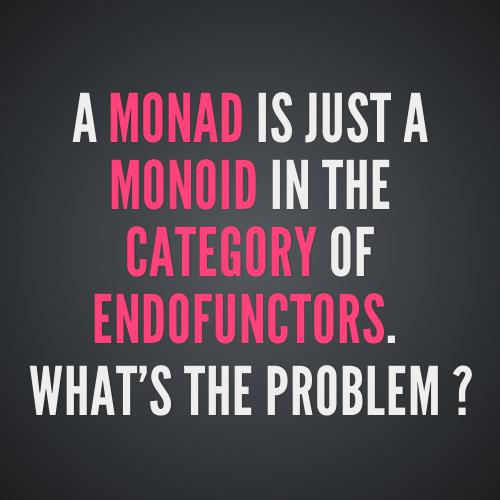
\includegraphics[height=0.9\textheight]{monad-is}}
\end{frame}

\end{comment}

\begin{frame}[fragile]
  \frametitle{Kleisli category}
  \begin{itemize}
    \item Kleisli categories formalise monadic composition
  \item For any monad $T$ over a category $\mathcal{C}$, the \alert{Kleisli category} of $\mathcal{C}$, written $\mathcal{C}_T$ is a category with the same objects as $\mathcal{C}$, but with morphisms given by:
    \begin{itemize}
    \item $\operatorname{hom}_{\mathcal{C}_T}(x,y) = \operatorname{hom}_\mathcal{C}(x,T(y)),\ \forall x,y\in\operatorname{ob}(\mathcal{C})$
    \end{itemize}
  \item The identity morphisms in $\mathcal{C}_T$ are given by $\operatorname{id}_x = \eta(x), \forall x$, and morphisms $f: x\longrightarrow T(y)$ and $g: y\longrightarrow T(z)$ in $\mathcal{C}$ can compose to form $g\, \circ_T f : x\longrightarrow T(z)$ via
    \begin{itemize}
      \item $g\ \circ_T f = \mu_z \circ T(g) \circ f$
    \end{itemize}
    leading to composition of morphisms in $\mathcal{C_T}$.
    \item In FP, the morphisms in $C_T$ are often referred to as \alert{Kleisli arrows}, or \alert{Kleislis}, or sometimes just \alert{arrows} (although \alert{Arrow} usually refers to a generalisation of Kleisli arrows, sometimes known as \alert{Hughes arrows})
  \end{itemize}
\end{frame}

\begin{comment}

\begin{frame}
\centerline{
\includegraphics[height=0.9\textheight]{say-monad}}
\end{frame}


\end{comment}

\begin{frame}[fragile]
  \frametitle{Comonads}
  \begin{itemize}
    \item The comonad is the categorical dual of the monad, obtained by ``reversing the arrows'' for the definition of a monad
  \item A \alert{comonad} on a category $\mathcal{C}$ is an endofunctor $W: \mathcal{C}\longrightarrow\mathcal{C}$ together with two natural transformations $\eps: W \longrightarrow \operatorname{Id}_\mathcal{C}$ (\alert{counit}) and $\delta: W\longrightarrow W^2$ (\alert{comultiplication}) fulfilling the \alert{comonad laws}:
    \begin{itemize}
    \item \alert{Associativity}: $\delta_W \circ \delta = W\delta \circ \delta$, as transformations $W\longrightarrow W^3$
      \item \alert{Identity}: $\eps_W \circ \delta = W\eps \circ \delta = 1_W$, as transformations $W\longrightarrow W$
    \end{itemize}
  \item The associativity law says that the two ways of \alert{duplicating} a $W(x)$ duplicated to a $W(W(x))$ to a $W(W(W(x)))$ are the same
  \item The identity law says that the two ways of \alert{extracting} a $W(x)$ from a $W(x)$ duplicated to a $W(W(x))$ are the same
  \end{itemize}
\end{frame}

\begin{comment}
  
\subsection{Scalable modelling and computation}

\begin{frame}[fragile]
  \frametitle{Laziness, composition, laws and optimisations}
  \begin{itemize}
    \item Laziness allows some optimisations to be performed that would be difficult to automate otherwise
    \item Consider a dataset |rdd: RDD[T]|, functions |f: T => U|, |g: U => V|, and a binary operation |op: (V,V) => V| for monoidal type |V|
    \item We can map the two functions and then reduce with:
      \begin{itemize}
      \item |rdd map f map g reduce op|
        \item to get a value of type |V|, all computed in parallel
      \end{itemize}
    \item However, re-writing this as:
      \begin{itemize}
      \item |rdd map (g compose f) reduce op|
        \item would eliminate an intermediate collection, but is equivalent due to the 2nd functor law (\alert{map fusion})
      \end{itemize}
      \item Category theory \alert{laws} often correspond to \alert{optimisations} that can be applied to code without affecting results --- Spark can do these optimisations \alert{automatically} due to lazy evaluation
  \end{itemize}
\end{frame}


\begin{frame}[fragile]
  \frametitle{Distributed computation}
  \begin{itemize}
  \item Big data frameworks such as Spark have been developed for the analysis of huge (internet scale) datasets on large clusters in the cloud
  \item They typically work by layering on top of a distributed file system (such as HDFS) which distributes a data set across a cluster and leaves data in place, sending required computation across the network to the data
    \item With a little thought, it is clear that even in the case of ``small data'' but ``big models''/``big computation'', these frameworks can be exploited for distributing computation
  \end{itemize}
\end{frame}

\end{comment}

\begin{frame}[fragile]
  \frametitle{Typeclasses}
  \begin{itemize}
  \item \alert{Typeclasses} are a mechanism for supporting \alert{ad hoc polymorphism} in (functional) programming languages
  \item They are more flexible way to provide polymorphic functionality than traditional inheritance-based object classes in conventional object-oriented programming languages
  \item To define a typeclass (such as |Monoid|) for a basic type, the language must support \alert{parametric types}
  \item To define a typeclass (such as |Functor| or |Monad|) for a parametric type or type constructor, the language must support \alert{higher-kinded types} (very few widely-used languages do)
  \end{itemize}
\end{frame}

\begin{frame}[fragile]
  \frametitle{Typeclasses for Monoid, Functor, Monad and Comonad}
%  \begin{itemize}
%  \item In Scala, we can define typeclasses for |Monoid|, |Functor| and |Monad| (using parametric and higher-kinded types):
%  \end{itemize}
  \begin{lstlisting}[language=scala]
  trait Monoid[A] {
    def combine(a1: A, a2: A): A
    def id: A
  }
  trait Functor[F[_]] {
    def map[A,B](fa: F[A])(f: A => B): F[B]
  }
  trait Monad[M[_]] extends Functor[M] {
    def pure[A](a: A): M[A]
    def flatMap[A,B](ma: M[A])(f: A => M[B]): M[B]
  }
  trait Comonad[W[_]] extends Functor[W] {
    def extract[A](wa: W[A]): A
    def coflatMap[A,B](wa: W[A])(f: W[A] => B): W[B] 
  }
\end{lstlisting}
\end{frame}

\begin{comment}
  
\begin{frame}[fragile]
  \frametitle{A generic collection typeclass}
  \begin{itemize}
  \item We can define a typeclass for generic monadic collections:
\begin{lstlisting}[language=scala]
trait GenericColl[C[_]] {
  def map[A,B](ca: C[A])(f: A => B): C[B]
  def flatMap[A,B,D[B] <: GenTraversable[B]](
                 ca: C[A])(f: A => D[B]): C[B]
  def reduce[A](ca: C[A])(f: (A, A) => A): A
  def zip[A,B](ca: C[A])(cb: C[B]): C[(A, B)]
  def length[A](ca: C[A]): Int
  ...
}
\end{lstlisting}
and then define instances for standard (serial) collections (eg. |Vector|), parallel collections (eg. |ParVector|), and distributed parallel collections (eg. |RDD|)
\item We can then write code that is completely \alert{parallelisation--agnostic}
  \end{itemize}
\end{frame}

\begin{frame}[fragile]
\frametitle{Scalable ABC}
\begin{itemize}
\item Simulate a collection of parameters, |pars: C[Param]|, from a prior and store in a generic collection
\item Define essential features of the ABC model:
\begin{lstlisting}[language=scala]
realData: Data    
simModel: Param => Data
summ: Data => SS
dist: (SS, SS) => Double
\end{lstlisting}
\item Then scalable (parallelism--agnostic) ABC is as simple as:
\begin{lstlisting}[language=scala]
val realSS = summ(realData)
pars.map(summ compose simModel).
  filter(dist(_, realSS) < eps)
\end{lstlisting}
using map--fusion to avoid constructing a collection of synthetic datasets
\end{itemize}
\end{frame}

\begin{frame}[fragile]
\frametitle{A scalable particle filter}
\begin{itemize}
  \item We can write a scalable particle filter by first writing a generic (parallel--agnostic) function to update a cloud of particles using a single observation, and then apply this to a sequence of observations
\end{itemize}
\begin{lstlisting}[language=scala]
  type PFState = GenericColl[State]

  val update: (PFState, Obs) => PFState = ???

  val data: Foldable[Obs] = ???
  val pi0: PFState = ???

  val piN = data.foldLeft(pi0)(update)
\end{lstlisting}
\end{frame}

  
\begin{frame}[fragile]
  \frametitle{A scalable particle filter}
Single--observation update of a bootstrap particle filter:
\begin{lstlisting}[language=scala]
def update[S: State, O: Observation,
  C[_]: GenericColl](
    dataLik: (S, O) => LogLik, stepFun: S => S,
    resample: (C[(Double, S)], Double, Int) => C[S]
  )( x: C[S], o: O): (LogLik, C[S] ) = {
    val xp = x map (stepFun(_))
    val lw = xp map (dataLik(_, o))
    val max = lw reduce (math.max(_, _))
    val rw = lw map (lwi => exp(lwi - max))
    val srw = rw reduce (_ + _)
    val l = rw.length
    val z = rw zip xp
    val rx = resample(z, srw, l)
    (max + log(srw / l), rx)
  }
\end{lstlisting}
\end{frame}

\begin{frame}[fragile]
\frametitle{Resampling}
Poisson resampling (for simplicity):
\begin{lstlisting}[language=scala]
def resamplePoisson[S: State, C[_]: GenericColl](
    zc: C[(Double,S)],
    srw: Double,
    l: Int
  ): C[S] = {
    zc flatMap {case (rwi, xpi) =>
      Vector.fill(Poisson(rwi * l / srw).draw)(xpi)
    }
  }
\end{lstlisting}
Resampling exploits the monadic nature of the collection (via |flatMap|)

Again, completely parallelisation--agnostic...
\end{frame}


\begin{frame}[fragile]
  \frametitle{Systematic resampling}
  Main body of systematic resampling algorithm:
\begin{lstlisting}[language=scala]
val W = w.scan(0.0)(_+_)
val rw = W map (_ * (l.toDouble / srw))
val u = Uniform(0,1).draw
val cumCount = rw map (x => {
  val f = math.floor(x).toInt
  if (u < x-f) (f+1) else f
})
val counts = diff(cumCount)
val cx = counts zip x
cx flatMap {case (ci, xi) => Vector.fill(ci)(xi)}
\end{lstlisting}
Again, no $\mathcal{O}(n)$ operations for parallel collections...
\end{frame}

\begin{frame}[fragile]
  \frametitle{Particle filtering as a functional fold}
 Once we have a function for executing one step of a particle filter, we can produce a function for particle filtering as a functional fold over a sequence of observations:
\begin{lstlisting}[language=scala]
val updater = update(dataLik, stepFun, resample) _
data.foldLeft((0.0, x0))((prev, o) => {
  val (oll, ox) = prev
  val (ll, x) = updater(ox, o)
  (oll + ll, x)
})
\end{lstlisting}
|foldLeft| is fundamentally sequential, but the |updater| is parallelisation-agnostic
\end{frame}


\begin{frame}[fragile]
\frametitle{Composable time series models}
\begin{itemize}
\item \alert{\url{git.io/statespace}} (Student: Jonny Law)
\item Scala library for nonlinear statespace modelling in continuous time for irregularly spaced observations on intractable Markov processes using particle filtering
  \item Compositional API for modelling building and use on-line with a streaming API based on Akka Streams
\end{itemize}
\begin{lstlisting}[language=scala]
val sde = Sde.brownianMotion(1)
val negBinModel = Model.negativeBinomial(sde)
val sde2 = Sde.ouProcess(8)
val composedMod = negBinModel |+|
  Model.seasonal(24, 4, sde2)
\end{lstlisting}
Another library: \alert{\url{git.io/dlm}} for more conventional linear state space modelling
\end{frame}

  
\begin{frame}[fragile]
\frametitle{Composable time series models}
\begin{itemize}
\item \alert{\url{git.io/dlm}} (Student: Jonny Law)
\item Library for more conventional discrete time DLMs and DGLMs with efficient filtering algorithms
\item Algebraic compositional structure to the API 
\end{itemize}
\begin{lstlisting}[language=scala]
val linear = Dlm.polynomial(1)
val seasonal = Dlm.seasonal(period=24, harmonics=3)
val regression = Dlm.regression(x=myTimeSeriesData)
val seasonalTrend = linear |+| seasonal
// model for a bivariate time series (cartesian)
val multivariateModel = linear |*| seasonalTrend
// model for 30 seemingly unrelated time series
val sutse = List.fill(30)(linear).reduce(_ |*| _)
// DGLMs
val poisson = Dglm.poisson(linear)
\end{lstlisting}
\end{frame}

\end{comment}

\begin{frame}[fragile]
  \frametitle{Comonads for statistical computation}
  \begin{itemize}
  \item Monads are good for operations that can be carried out on data points independently
    \item For computations requiring knowledge of some kind of local neighbourhood structure, \alert{Comonads} are a better fit
    \item |coflatMap| will take a function representing a \alert{local computation} producing one value for the new structure, and then extend this to generate all values associated with the comonad
      \item Useful for defining linear filters, Gibbs samplers, convolutional neural networks, etc.
    \end{itemize}
\end{frame}

\begin{comment}
  
\begin{frame}[fragile]
\frametitle{Linear filters for Streams and Images}  
Let's start with writing a function to compute the weighted average of values at the start of an infinite data |Stream|
\begin{lstlisting}[language=scala]
def linFilter(weights: Stream[Double])(
  s: Stream[Double]): Double =
  (weights, s).parMapN(_*_).sum    
\end{lstlisting}
We can extend this \alert{local computation} to the entire |Stream| using |coflatMap|
\begin{lstlisting}[language=scala]
s.coflatMap(linFilter(Stream(0.25,0.5,0.25)))
\end{lstlisting}
resulting in a new infinite |Stream| containing the filtered values
\begin{itemize}
\item  Note that the method |extract| will return the value at the head of the |Stream|
  \end{itemize}
\end{frame}

\begin{frame}[fragile]
\frametitle{Filtering an Image}
\begin{itemize}
\item For a 2D Image, the relevant context for local computation is less clear, so to become comonadic, the Image class needs to be ``pointed'', by augmenting it with a ``cursor'' pointing to the current pixel of interest
\item For the pointed image class, |extract| returns the value of the pixel at the cursor
\item We filter using functions which compute a value on the basis of the ``neighbourhood'' of the cursor
\item |map| and |coflatMap| operations will automatically parallelise if the image is backed with a parallel data structure
\end{itemize}
\begin{lstlisting}[language=scala]
def fil(pi: PImage[Double]):Double = (2*pi.extract+
  pi.up.extract+pi.down.extract+
  pi.left.extract+pi.right.extract)/6.0
val filteredImage = pim0.coflatMap(fil)  
def pims = Stream.iterate(pim0)(_.coflatMap(fil))
\end{lstlisting}
\end{frame}

\begin{frame}[fragile]
\frametitle{Gibbs sampling (an Ising model)}
\begin{lstlisting}[language=scala]
def gibbsKernel(pi: PImage[Int]): Int = {
   val sum = pi.up.extract+pi.down.extract+
     pi.left.extract+pi.right.extract
   val p1 = math.exp(beta*sum)
   val p2 = math.exp(-beta*sum)
   val probplus = p1/(p1+p2)
   if (new Bernoulli(probplus).draw) 1 else -1
}
def oddKernel(pi: PImage[Int]): Int =
  if ((pi.x+pi.y) % 2 != 0) pi.extract else
    gibbsKernel(pi)
def evenKernel(pi: PImage[Int]): Int =
  if ((pi.x+pi.y) % 2 == 0) pi.extract else
    gibbsKernel(pi)
def pims=Stream.iterate(pim0)(_.coflatMap(oddKernel).
  coflatMap(evenKernel))
\end{lstlisting}
\end{frame}


\begin{frame}
  \frametitle{Recursion schemes}
  \begin{itemize}
  \item A \alert{fold} over a sequential data structure is an example of a recursion scheme known more formally as a \alert{catamorphism} (eg. sums and AD)
  \item The generation of a sequential stream of values from a seed and a generation function (eg. the generation of an MCMC chain) is an example of an \alert{unfold} operation, more formally known as an \alert{anamorphism}
    \item Generating and then consuming a data structure (eg. simulating an MCMC chain and then computing summary statistics from the iterations) is an example of a \alert{refold}, known formally as a \alert{hylomorphism}
  \end{itemize}
  (glossing over \alert{F-algebras}, \alert{coalgebras}, \alert{ADTs} and \alert{fixed point types})
  \medskip
  
  Again, category theory provides the theory and FP languages provide frameworks and abstractions for implementation
\end{frame}


\begin{frame}[fragile]
  \frametitle{Scalable statistical modelling}
  \begin{itemize}
  \item We have looked a lot at scalable statistical \alert{computation}, but what about scalable statistical \alert{modelling} more generally?
  \item Independently of any computational issues, statistical modelling of large, complex problems is all about structure, modularity and composition --- again, the domain of category theory...
  \item When Bayesian hierarchical modelling, we often use \alert{probabilistic programming languages} (such as BUGS, JAGS, Stan...) to build up a large, complex (DAG) model from simple components
    \item It turns out that \alert{monads}, and especially \alert{free monads}, can give us a different (better?) perspective on building and inferring probabilistic models
  \end{itemize}
\end{frame}

\end{comment}

\section{Probability monads}

\subsection{Composing random variables}

\begin{frame}[fragile]
  \frametitle{Composing random variables with the probability monad}
  \begin{itemize}
  \item The \alert{probability monad} provides a foundation for describing random variables in a pure functional way (cf. \alert{Giry monad})
  \item We can build up joint distributions from marginal and conditional distributions using \alert{monadic composition}
  \item For example, consider an exponential mixture of Poissons (marginally negative binomial): we can think of an exponential distribution parametrised by a rate as a function |Exponential: Double => Rand[Double]| and a Poisson parametrised by its mean as a function |Poisson: Double => Rand[Int]|
    \item Those two functions don't directly compose, but do in the Kleisli category of the |Rand| monad, so |Exponential(3) flatMap {Poisson(_)}| will return a |Rand[Int]| which we can draw samples from if required
  \end{itemize}
\end{frame}


\begin{frame}[fragile]
  \frametitle{Monads for probabilistic programming}
  \begin{itemize}
    \item For larger probability models we can use \alert{for-comprehensions} to simplify the model building process, eg.
\begin{lstlisting}[language=scala]
  for { mu <- Gaussian(10,1)
        tau <- Gamma(1,1)
        sig = 1.0/sqrt(tau)
        obs <- Gaussian(mu,sig) }
  yield ((mu,tau,obs))
\end{lstlisting}
  \item We can use a regular probability monad for building forward models this way, and even for building models with simple Bayesian inference procedures allowing conditioning
    \item For sophisticated probabilistic sampling algorithms (eg. SMC, MCMC, pMCMC, HMC, ...) and hybrid compositions, it is better to build models like this using a \alert{free monad} which can be \alert{interpreted} in different ways
  \end{itemize}
\end{frame}

\begin{comment}

\begin{frame}[fragile]
\frametitle{MCMC as a Stream}
\begin{itemize}
\item Impure:
\begin{lstlisting}[language=scala]
def nextState(oldState: State): State = ???

Stream.iterate(initialState)(nextState).
  drop(1000).thin(10).take(10000)
\end{lstlisting}
Note that |iterate| is to |unfold| as |reduce| is to |fold|
\item Pure:
\begin{lstlisting}[language=scala]
def kernel(oldState: State): Rand[State] = ???

MarkovChain(initialState)(kernel).steps.
  drop(1000).thin(10).take(10000)
\end{lstlisting}
\end{itemize}
\end{frame}

\end{comment}

\begin{frame}
  \frametitle{Probability monad foundations}
  Mathematically, what \alert{exactly} is a probability monad $P$\,?

  Standard answer:
  
  \begin{itemize}
  \item \alert{Giry monad} --  measurable functions and spaces
    \begin{itemize}
      \item Defined on the category \textbf{Meas} of measurable spaces, $P$ sends $X$ to the space of probability measures on $X$
      \item $\eta$ is a dirac measure ($\eta(x) = \delta_x$) and $\mu$ is defined as marginalisation using Lebesgue integration
        \[
\mu_X(\rho)(A) = \int_{P(X)} \tau_A(d\rho)
        \]
      \item Provides a solid foundation matching up closely with conventional probability theory, but isn't as compositional as we'd like (eg. \textbf{Meas} is not cartesian closed)
        \item Awkward for (higher--order) probabilistic programming languages
    \end{itemize}
  \end{itemize}
\end{frame}

\begin{frame}
  \frametitle{Alternative probability monad foundations}
  \begin{itemize}
\item \alert{Quasi-Borel spaces}
    \begin{itemize}
    \item A modification of the measure space approach which is cartesian closed (eg. $\reals^\reals = \mathbf{QBS}(\reals,\reals)$)
      \item Good for the denotational semantics of (higher--order) probabilistic programming languages where we want to define probability distributions over functions
    \end{itemize}
  \item \alert{Kantorovich monad} -- built on (complete) metric spaces
    \begin{itemize}
\item Provides an alternative, more composable foundation for probability theory, less tightly linked to measure theory
    \end{itemize}
  \item \alert{Expectation monad} -- directly define an expectation monad
    \begin{itemize}
      \item A formulation in which expectation is primitive and probability is a derived concept (cf. de Finetti)
    \end{itemize}
  \end{itemize}
And several others...
\end{frame}

\begin{comment}

%\subsection{Monads for UQ}

\begin{frame}[fragile]
  \frametitle{Probability monads for uncertainty quantification (UQ)}
  \begin{itemize}
  \item Suppose we have a \alert{computer model}, $f$, mapping inputs (or parameters) $x\in X$ to output $y\in Y$:
    \[
    f: X \longrightarrow Y
    \]
  \item Suppose further that we are uncertain about the ``correct'' inputs to use, and encapsulate our uncertainty in a probability distribution $p_X \in P(X)$, where $P$ denotes a probability monad
  \item We can't apply $f$ to $p_X$ (the types don't match), but we can use the fact that $P$ is a functor to ``lift'' $f$ into the monad (|px map f|):
    \[
    P(f): P(X) \longrightarrow P(Y),
    \]
    inducing a probability distribution on the output.
  \end{itemize}
\end{frame}


\begin{frame}[fragile]
  \frametitle{UQ for stochastic computer models}
  \begin{itemize}
  \item Suppose now that we have a stochastic (non-deterministic) computer model (or emulator):
    \[
g: X \longrightarrow P(Y),
\]
so that for an given fixed input $x\in X$, the output is a probability distribution over $Y$
\item If we have additional uncertainty for the input $x\in X$, then we lift $g$ into the Kleisli category of the monad (|px flatMap g|):
  \[
  \mu_Y\circ P(g): P(X) \longrightarrow P(Y),
  \]
  effectively just marginalising over our uncertainty about $x$
  \end{itemize}
\end{frame}

\end{comment}

\subsection{Implementations of probability monads}

\begin{frame}[fragile]
  \frametitle{\texttt{Rand} for forward simulation}
  \begin{itemize}
    \item Whilst the semantics of probability monads should be reasonably clear, there are many different ways to implement them, depending on the intended use-case
  \item The simplest probability monad implementations typically provide a |draw| method, which can be used (with a uniform random number generator) to generate draws from the distribution of interest
  \item For |x: Rand[X]|, monadic bind |x flatMap (f: X => Rand[Y])| returns |y: Rand[Y]|
    \item |f| represents a conditional distribution and |y| represents the marginalisation of this distribution over |x|
    \item The |draw| method for |y| first calls |draw| on |x| (which it holds a reference to), feeds this in to |f| and then calls |draw| on the result
    \end{itemize}
\end{frame}

\begin{comment}
  
\begin{frame}
  \frametitle{\texttt{Gen} for property-based testing}
  \begin{itemize}
  \item It turns out that monads representing non-determinism are widely used for software testing in FP languages
  \item Property-based testing is an alternative to unit testing, and is concerned with specifying the properties that your function should satisfy rather than focusing on specific test cases
  \item Having specified the properties, the testing library then randomly generates test cases for stress-testing functions to ensure correct behaviour
  \item While not representing a true probability monad (distributional properties are unspecified), these generators have much in common with forward simulation probability monads
    \item \texttt{ScalaCheck} in Scala and \texttt{QuickCheck} in Haskell are well-known examples of property-based testing libraries
    \end{itemize}
\end{frame}

\end{comment}

\begin{frame}[fragile]
  \frametitle{\texttt{Dist} for Bayesian conditioning via SMC}
  \begin{itemize}
  \item Rather than providing a |draw| method for generating individual values from the distribution of interest, you can define a monad whose values represent large (weighted) random samples from a distribution --- an empirical distribution
  \item |flatMap| is then essentially just the same |flatMap| you would have on any other collection, but here will typically be combined with a random thinning of the result set to prevent an explosion in the number of particles with deep chaining
  \item One advantage of this representation is that it then easy to introduction a |condition| method which uses importance (re)sampling to condition on observations
    \item This can be used to implement a simple SMC-based Bayesian PPL with very little code, but it won't scale well with large or complex models
    \end{itemize}
\end{frame}

\begin{frame}[fragile]
  \frametitle{\texttt{RandomVariable} for Bayesian HMC sampling}
  \begin{itemize}
  \item Rather than using a probability monad to represent samples or methods for sampling, one can instead use them to represent the (joint, log) density of the variables
    \item |flatMap| just multiplies the (conditional) densities
    \item Again, conditioning is easy (multiplication), so this forms a good basis for Bayesian PPLs
    \item Can use the joint posterior for simple MH algorithms (and Gibbs, if dependencies are tracked), but for Langevin and HMC algorithms, also need to keep track of gradients, using automatic differentiation (AD)
      \item OK, because (reverse-mode) AD on a compute graph is also monadic!
    \item \alert{Rainier} is a Scala library for HMC sampling of monadic random variables (using a static compute graph, for efficiency)
    \end{itemize}
\end{frame}

\subsection{Probabilistic programming}

\begin{frame}[fragile]
\frametitle{Example --- Bayesian logistic regression model in Rainier}
\begin{lstlisting}[language=scala]
val model = for {
      beta0 <- Normal(0, 5).param
      beta1 <- Normal(0, 5).param
      _ <- Predictor.fromDouble { x =>
          {
            val theta = beta0 + beta1 * x
            val p = Real(1.0) / (Real(1.0) +
                (Real(0.0) - theta).exp)
            Categorical.boolean(p)
          }
        }.fit(x zip y)
} yield Map("b0" -> beta0, "b1" -> beta1)

val out = model.sample(HMC(5), 1000, 10000*10, 10)
\end{lstlisting}
\end{frame}

\begin{frame}
  \frametitle{Composing probabilistic programs}
  \begin{itemize}
  \item Describing probabilistic programs as \alert{monadic values} in a functional programming language with syntax for monadic composition leads immediately to an \alert{embedded PPL DSL} ``for free''
  \item This in turn enables a fully \alert{compositional} approach to the (scalable) development of (hierarchical) probabilistic models
  \item Model components can be easily ``re-used'' in order to build big models from small
  \item eg. a regression model component can be re-used to create a hierarchical random effects model over related regressions
    \item In some well-known PPLs (eg. BUGS), this would require manual copy-and-pasting of code, wrapping with a ``for loop'', and manual hacking in of an extra array index into all array references --- not at all compositional!
  \end{itemize}
\end{frame}


\begin{frame}[fragile]
  \frametitle{Representation independence using the \emph{free} monad}
  \begin{itemize}
  \item However you implement your probability monad, the semantics of your probabilistic program are (essentially) the same
  \item It would be nice to be able to define and compose probabilistic programs independently of concerns about implementation, and then to \alert{interpret} the program with a particular implementation later
  \item Building a probability monad on top of the \alert{free monad} allows this --- implementation of |pure| and |flatMap| is ``suspended'' in a way that allows subsequent interpretation with concrete implementations later
    \item This allows \alert{layering} of multiple inference algorithms, and different interpretation of different parts of the model, enabling sophisticated \alert{composition} of different (hybrid) inference algorithms
    \end{itemize}
\end{frame}


\begin{comment}
  
\begin{frame}
  \frametitle{Bayesian hierarchical models, graphical models and probabilistic programs}
  \begin{itemize}
  \item Bayesian hierarchical models are one of the most powerful tools we have for understanding large and complex data sets --- their hierarchical nature makes them naturally compositional
  \item Bayesian graphical models are also quite compositional, and can often be used to represent Bayesian hierarchical models
  \item Bayesian hierarchical and graphical models can be modelled as probabilistic programs, so probabilistic programming can be used as a unifying framework for describing (Bayesian) statistical models
    \item We want our probabilistic programming languages to be compositional (functional and monadic?), in order to naturally scale with model size and complexity
  \end{itemize}
\end{frame}

\end{comment}

\begin{frame}
  \frametitle{Compositionality of inference algorithms}
  \begin{itemize}
  \item As well as building \alert{models} in scalable, compositional way, we would also like our \alert{inference algorithms} to be compositional, ideally reflecting the compositional structure of our models
  \item Some algorithms, such as component-wise samplers and message-passing algorithms, naturally reflect the compositional structure of the underlying model
  \item Other algorithms, such as Langevin and HMC samplers, deliberately don't decompose with the model structure, but do have other structure that can be exploited, such as decomposing over observations
    \item Understanding and exploiting the \alert{compositional structure} of models and algorithms will be crucial for developing scalable inferential methods
  \end{itemize}
\end{frame}



\section{Summary and conclusions}

%\subsection{Summary}

\begin{frame}
  \frametitle{Summary}
  \begin{itemize}
  \item Mathematicians and theoretical computer scientists have been thinking about models of (scalable) computation for decades
  \item \alert{Functional programming languages} based on Cartesian closed categories provide a sensible foundation for computational modelling with appropriate levels of abstraction
  \item Concepts from \alert{category theory}, such as functors, monads and comonads, provide an appropriate array of tools for scalable data modelling and algorithm construction and composition
    \item Expressing models and algorithms in FP languages using category theory abstractions leads to \alert{elegant, composable PPLs ``for free''}, doing away with the need to manually construct and parse custom DSLs
\item Monadic composition is \alert{the} \emph{canonical} approach to constructing flexible, composable PPLs (and AD systems, and deep NNs, ...)
  \end{itemize}
\end{frame}


\begin{comment}

\begin{frame}
  \frametitle{Summary}
  \begin{itemize}
  \item You can't learn much about either FP or CT in a single talk/seminar
  \item I don't expect everyone to have understood everything!
  \item The aim was to give a little insight into:
    \begin{itemize}
    \item Why FP is interesting, and inherently more modular, composable and scalable than imperative programming
    \item Why CT is a good model for composable computation (because it is a theory of structure and composition)
      \item Why CT provides powerful abstractions which make FP easier, more modular, and more general
      \end{itemize}
  \end{itemize}
\end{frame}


\subsection{Conclusions}

\frame{
  \frametitle{Conclusions}
  \begin{itemize}
  \item We should approach the problem of statistical modelling and computation in a modular, composable, functional way, guided by underpinning principles from category theory
  \item To implement solutions to problems in statistical modelling and computation in a more scalable way, we need programming languages which are:
    \begin{itemize}
    \item \alert{Strongly statically typed}
    \item \alert{Compiled}
    \item \alert{Functional}
      \item and support \alert{concurrency}, \alert{parallelism}, \alert{typeclasses} and \alert{higher-kinded types}
    \end{itemize}
  \item \alert{Scala} and \alert{Spark} provide a nice illustration of the power of this approach, but there are other interesting languages, including: Haskell, Idris, OCaml, Frege, Eta, PureScript, \ldots
  \end{itemize}
  }

\end{comment}

\begin{frame}
  \frametitle{References}

  \setbeamerfont{bibliography item}{size=\footnotesize}
  \setbeamerfont{bibliography entry author}{size=\footnotesize}
  \setbeamerfont{bibliography entry title}{size=\footnotesize}
  \setbeamerfont{bibliography entry location}{size=\footnotesize}
  \setbeamerfont{bibliography entry note}{size=\footnotesize}
  
  \begin{thebibliography}{}

%  \bibitem{} Elliott, C. (2017) \alert{Generic functional parallel algorithms: Scan and FFT}. \emph{ICFP 2017}, \textbf{1}:7.

\bibitem{} Fong, B., Spivak, D., Tuy\'eras, R. (2019) \alert{Backprop as Functor: A compositional perspective on supervised learning}, \emph{arXiv}, 1711.10455
   
%   \bibitem{} Fritz, T., Perrone, P. (2017) \alert{A probability monad as the colimit of finite powers}, \emph{arXiv:1712.05363}.

\bibitem{} Heunen, C., Kammar, O., Staton, S., Yang, H. (2017) \alert{A convenient category for higher-order probability theory}, \emph{32nd ACM/IEEE LICS.}, 1--12.
     
    \bibitem{} Law, J., Wilkinson, D. J. (2018) \alert{Composable models for online Bayesian analysis of streaming data}, \emph{Statistics and Computing}, \textbf{28}(6):1119--1137.
    
%    \bibitem{} Meijer, E., Fokkinga, M., Paterson, R. (1991) \alert{Functional programming with bananas, lenses, envelopes and barbed wire}. In: Hughes J. (eds) \emph{Functional Programming Languages and Computer Architecture}. FPCA 1991. Lecture Notes in Computer Science, vol 523. Springer.

    \bibitem{} Park, S., Pfenning, F., Thrun, S. (2008) \alert{A probabilistic language based on sampling functions}, \emph{TOPLAS}, \textbf{31}(1):4.

\bibitem[\protect\citeauthoryear{blah}{blah}{2011}]{blah} \'{S}cibior, A., Ghahramani, Z. and Gordon, A. D. (2015) \alert{Practical probabilistic programming with monads}, \emph{Proceedings of the 2015 ACM SIGPLAN Symposium on Haskell}, 165--176.

\bibitem{} \'{S}cibior, A., Kammar, O., Gharamani, Z. (2018) \alert{Functional programming for modular Bayesian inference}, \emph{Proc.\ ACM Prog.\ Lang.}, \textbf{2}(ICFP): 83.
      
%  \bibitem[\protect\citeauthoryear{blah}{blah}{2011}]{blah} \'{S}cibior, A. et al (2018) \alert{Denotational validation of higher-order Bayesian inference}, \emph{Proc.\ ACM Prog.\ Lang.}, \textbf{2}(POPL): 60.
    
%     \bibitem{} Wadler, P. (1995) \alert{Monads for functional programming}. In: Jeuring J., Meijer E. (eds) \emph{Advanced Functional Programming}. AFP 1995. Lecture Notes in Computer Science, vol 925. Springer.
    
%\beamertemplatebookbibitems
%
%\bibitem[\protect\citeauthoryear{blah}{blah}{2011}]{blah} Barr, M. and Wells, C. (1990) \alert{Category Theory for Computing Science}, Prentice Hall.
    
  \end{thebibliography}

  \vspace*{0.8ex}

  Rainier:
  \alert{\url{github.com/stripe/rainier}}

%  For more about Scala and FP: \alert{\url{darrenjw.wordpress.com}}

 \alert{\url{darrenjw.github.io}} \hfill \url{@darrenjw}
  
\end{frame}



\end{document}

